\chapter{Konzept Web}

\label{konzept_web}
\section{Allgemein}

Unsere Dienstleistung konzentriert sich ähnlich der Unix Philosophie auf eine
bestimmte Tätigkeit und versucht diese möglichst gut zu realisieren. Aufgrund
dieser Tatsache ist es uns sehr wichtig den User nicht mit ,,Thematikfremden''
Themen zu nerven. Aufgrund unserer Spezialisierung werden fachfremde Kategorien
wie z.B. der Fanartikel Webshop an Drittanbieter ,,outgesourct''.
\\
\\
Um eine einfache sowie angenehme Usability zu gewährleisten konzentrieren wir
uns sehr stark darauf das \emph{Design} nach dem KISS-Prinzip so einfach wie
möglich zu halten und den Benutzer nicht mit Werbebannern oder sinnfreien
Informationen zu belästigen.

\newpage

\section{Farbklima}
Das an den Key-Visual angepasste Farbklima sieht wie folgt aus:

\begin{table}[h!]
\centering
\begin{tabular*}{\textwidth}{lll|l}

    Farbe & Name & Farbwerte & Einsatzgebiet \\
    \hline
    
\multirow{3}{*}
    {
    \begin{tikzpicture}
        \draw [line width=0.5pt,fill=a]
        (0,0) -- (1.2,0) -- (1.2,1.2) -- (0,1.2) -- cycle;
    \end{tikzpicture}
    }
    & a & HEX \#FDF9EF & Hintergrundfarbe für Contentbereich\\
    & & RGB 253, 249, 239 \\
    & &  \\
    \hline

\multirow{3}{*}
    {
    \begin{tikzpicture}
        \draw [line width=0.5pt, fill=b]
        (0,0) -- (1.2,0) -- (1.2,1.2) -- (0,1.2) -- cycle;
    \end{tikzpicture}
    }
    & b & HEX \#F4F1E5 &  Hintergrund \\ 
    & & RGB  244, 241, 229 & \\
    & &  \\
    \hline

\multirow{3}{*}
    {
    \begin{tikzpicture}
        \draw [line width=0.5pt,fill=c]
        (0,0) -- (1.2,0) -- (1.2,1.2) -- (0,1.2) -- cycle;
    \end{tikzpicture}
    }
    & c & HEX \#544738 &  Standard Schriftfarbe \\
    & & RGB 84, 71, 56 & \\
    & &  \\
    \hline

\multirow{3}{*}
    {
    \begin{tikzpicture}
        \draw [line width=0.5pt,fill=d]
        (0,0) -- (1.2,0) -- (1.2,1.2) -- (0,1.2) -- cycle;
    \end{tikzpicture}
    }
    & d & HEX \#98BF21 &   Buttonflächen \\
    & & RGB 152, 191, 33 & \\
    & &  \\
    \hline

\multirow{3}{*}
    {
    \begin{tikzpicture}
        \draw [line width=0.5pt,fill=e]
        (0,0) -- (1.2,0) -- (1.2,1.2) -- (0,1.2) -- cycle;
    \end{tikzpicture}
    }
    & e & HEX \#C2C5BE &  Footer Hintergrundfarbe \\
    & & RGB 194, 197, 190 &\\ 
    & &  \\
    \hline
   
\multirow{3}{*}
    {
    \begin{tikzpicture}
        \draw [line width=0.5pt,fill=f]
        (0,0) -- (1.2,0) -- (1.2,1.2) -- (0,1.2) -- cycle;
    \end{tikzpicture}
    }
    & f & HEX \#BBBBBB &  Tagcloud Schriftfarbe \\
    & & RGB 187, 187, 187  & \\
    & &  \\
    \hline
   
\multirow{3}{*}
    {
    \begin{tikzpicture}
        \draw [line width=0.5pt,fill=g]
        (0,0) -- (1.2,0) -- (1.2,1.2) -- (0,1.2) -- cycle;
    \end{tikzpicture}
    }
    & g & HEX \#303030 &  Tagcloud Farbe \\
    & & RGB 48, 48, 48  & \\
    & &  \\

\end{tabular*}
   \caption{Farbschema}
   \label{t_colorscheme}
\end{table}

\section{Webservice Kategorien}
Folgende Hauptkategorien wurden auf moosr umgesetzt:

\newpage

\paragraph{Layoutübersicht}

\label{moosrdata_ref}
\begin{center}
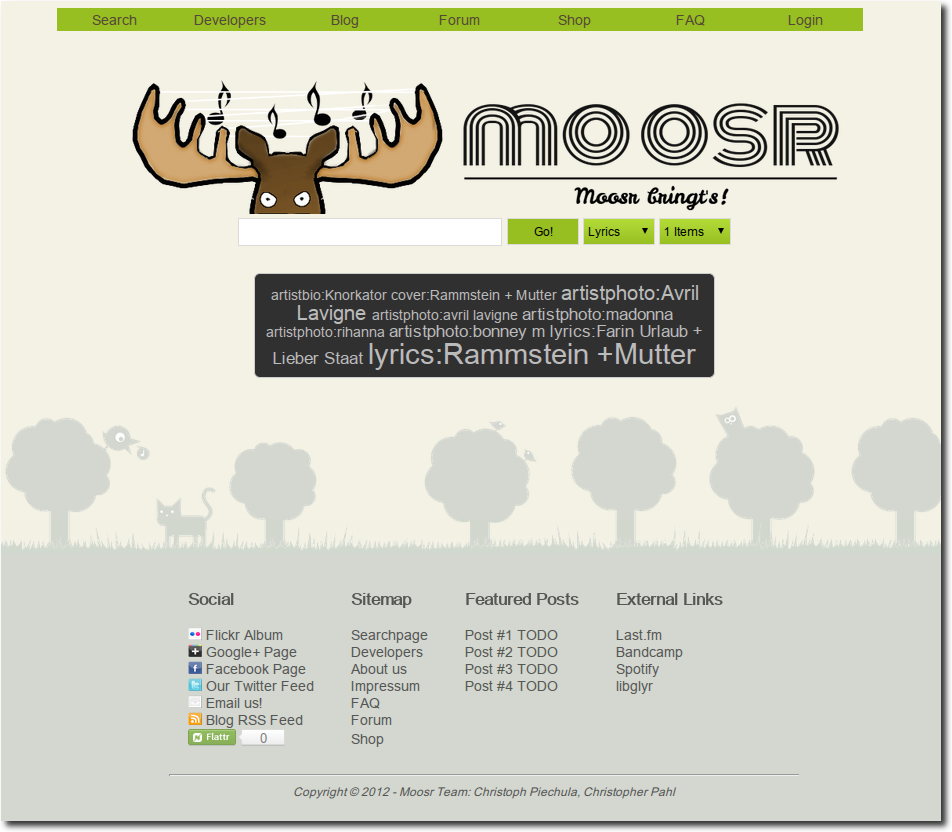
\includegraphics[width=\textwidth]{../screenshots/moosrdata.png}
\end{center}

\paragraph{moosrdata}
Hier befindet sich die der Kernpunkt unserer Dienstleistung, die Metadaten
Suchmaschine. Diese Seite bietet dynamischen Content in Form einer
\emph{Tagcloud} mit den zu einem bestimmten Zeipunkt am häufigsten gesuchtenn
Metadaten. Die Suche ist auch in der Übersicht unter \ref{moosrdata_ref}
gezeigt.
\\
\\
Bei einer Suche wird ein angepasstes Layout angezeigt. 
Hier als Beispiel das Layout bei der Anzeige von Coverart:

\begin{center}
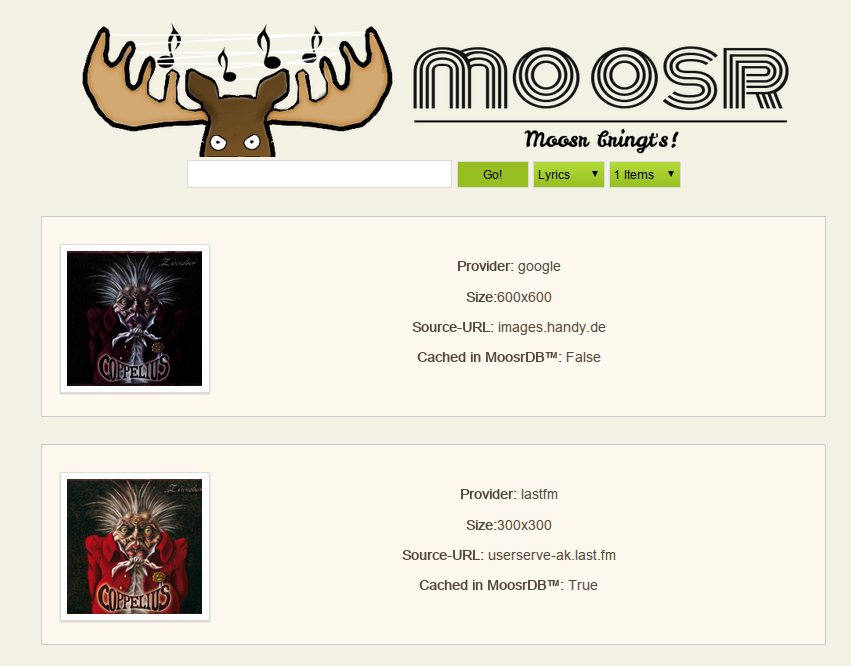
\includegraphics[width=\textwidth]{../screenshots/moosrdata_cover_results.png}
\end{center}

Textuelle Resultate werden folgendermaßen angezeigt:
\begin{center}
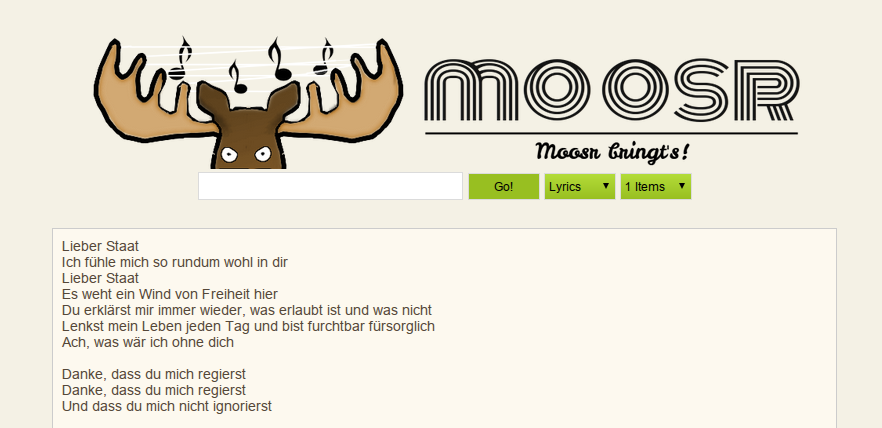
\includegraphics[width=\textwidth]{../screenshots/moosrdata_lyrics_results.png}
\end{center}


\newpage
\paragraph{Developers}
\label{static_page}
\begin{center}
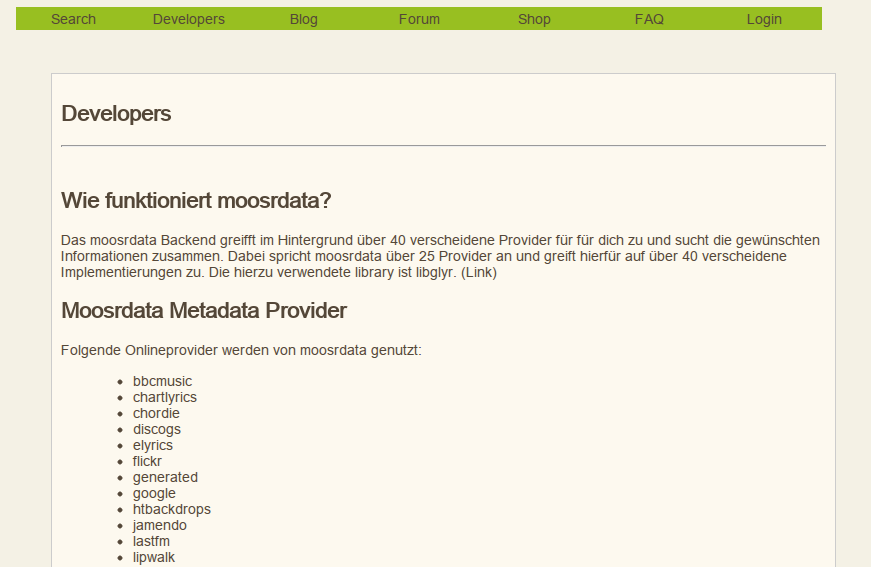
\includegraphics[width=\textwidth]{../screenshots/developers.png}
\end{center}

Die Kategorie \emph{Developers} ist eine Seite mit statischem Content. Hier
werden für interessierte Entwickler alle Informationen zu unserer HTML
Darstellung und JSON API erläutert.

\paragraph{Blog}
Der \emph{Blog} ist eine Seite mit wachsendem Content. Über diese Seite wollen
wir unsere Community auf dem Laufenden halten über Newcomer aus der Szene und
Berichte über Alben, Festivals etc. verfassen. Die ,,Blogsoftware'' wurde von
uns in Flask implementiert damit diese die SEO Anforderungen optimal beherrscht.
\\
\\
Die Loginmaske erlaubt ein SEO-gerechtes Eintragen von Artikeln:
\begin{center}
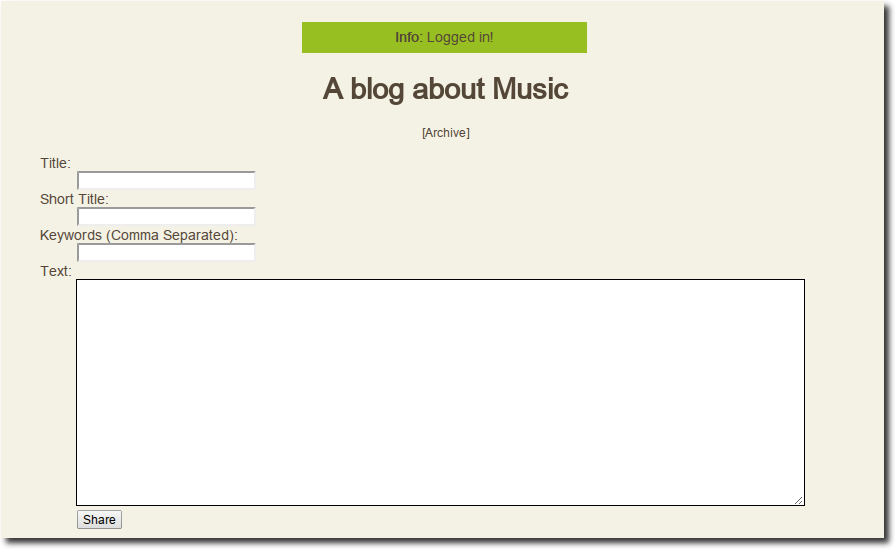
\includegraphics[width=\textwidth]{../screenshots/post_entry.png}
\end{center}
\label{blog_post_mask}

Die Beiträge sind dabei in reStructuredText zu verfassen. Beim Posten werden
diese zu HTML konvertiert. Hierbei ergibt sich ein fest vorgegebenes Header
Schema was eine manuelle Definition der Header überflüssig macht.
Siehe dazu die reStructuredText Dokumentation:

\begin{center}
\url{http://docutils.sourceforge.net/docs/user/rst/quickstart.html}
\end{center}
Momentan enthält der \emph{Blog} vier von uns verfasste Beiträge die ebenfalls gut von Google
gerankt werden sollen. Hierbei wurde darauf geachtet, dass ein primäres und
mehrere sekundäre Keywords wie gewünscht festgelegt wurden und diese mehrmals im
Text wiederholt wurden. Diese wurden beim Verfassen des Blogeintrags als
Keywords festgelegt und somit vom Blogsystem als Meta-Keywords in den HTML
Quelltext geschrieben.

\begin{verbatim}
    <meta name="keywords" content="Coppelius, Band, Kammercore, Klassik" />
\end{verbatim}

Es folgt ein Screenshot der Blogübersicht. Es wird nicht der vollständige
Beitrag angezeigt sondern jeweils nur ein Bild und ein Teaser:

\begin{center}
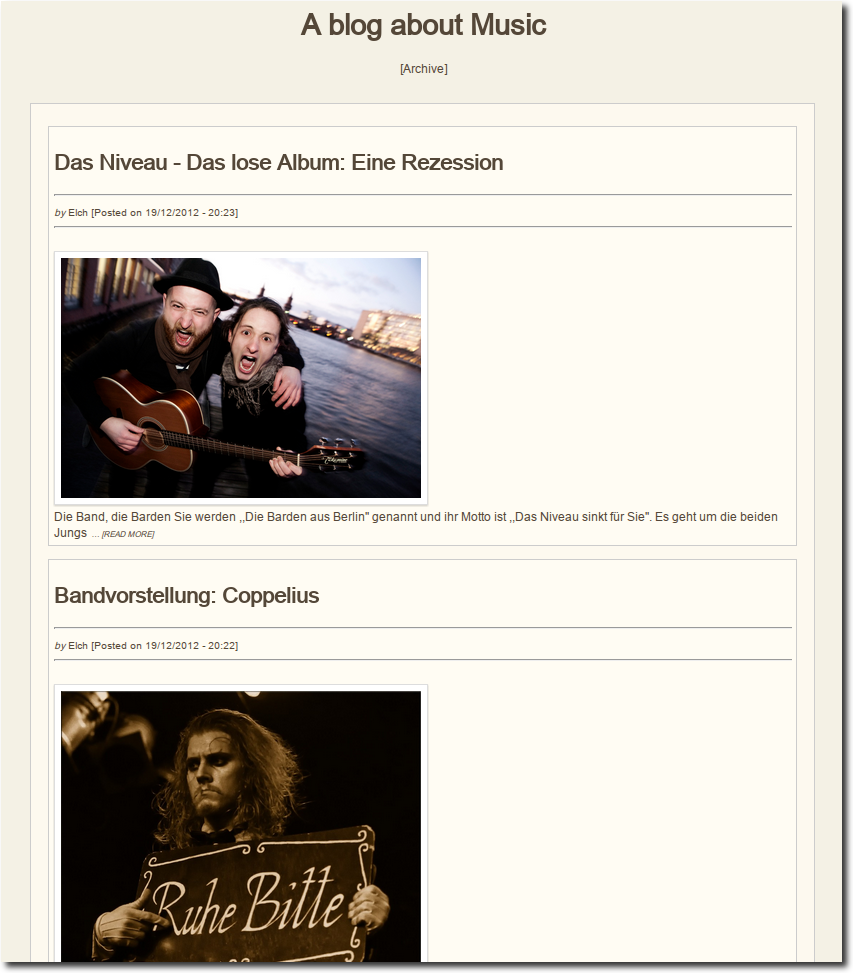
\includegraphics[width=\textwidth]{../screenshots/blog_overview.png}
\end{center}

In der Übersicht ist die Detailansicht des Beitrags verlinkt. Darin ist der
vollständige Beitrag sichtbar: 

\begin{center}
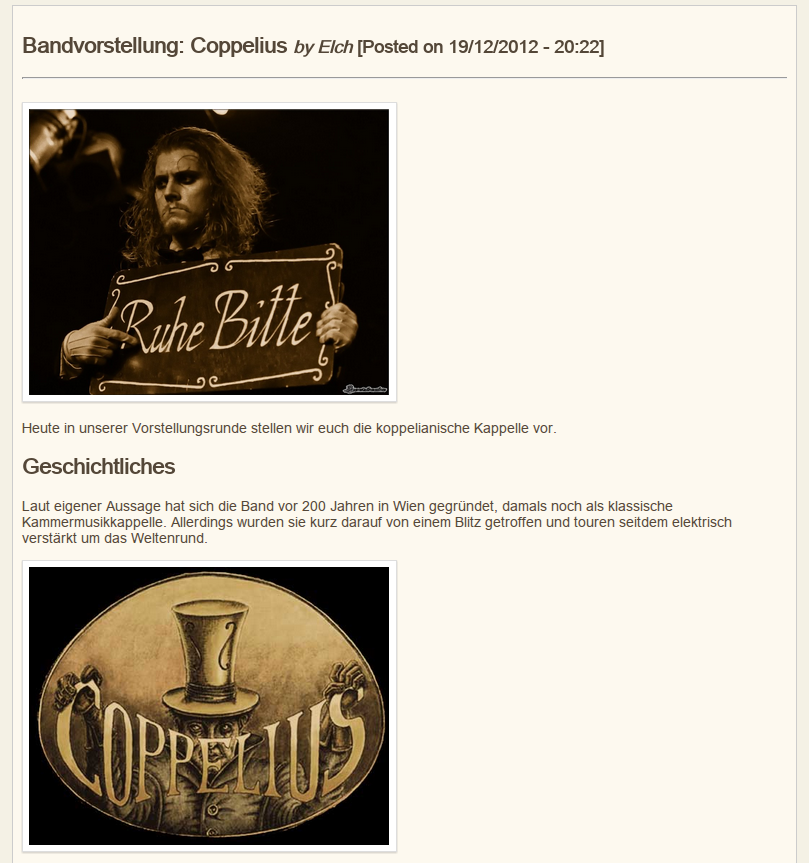
\includegraphics[width=\textwidth]{../screenshots/blog_detail.png}
\end{center}

Das Archiv bietet eine Übersicht über alle vorhanden Posts, und listet das
Datum, den Autor, den Kurztitel sowie die Keywords auf. Durch das Archiv sollen
auch ältere, nicht mehr andersweitig verlinkte Posts Linkkraft erhalten.

\begin{center}
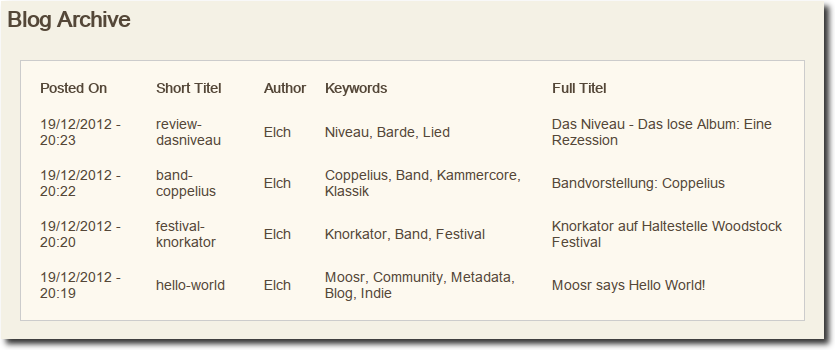
\includegraphics[width=\textwidth]{../screenshots/blog_archive.png}
\end{center}

\paragraph{Webshop}
In der Kategorie \emph{Webshop} befinden sich Seitenlinks und Beschreibungen zu
Webshops mit Tickets und Fanartikeln. Diese Seite enthält hauptsächlich
statischen Content, daher wurde auf einen Screenshot verzichtet. Siehe
\ref{static_page}.

\paragraph{Forum}
Das \emph{Forum} ist der Haupttreffpunkt für die Community. Hier können sich
alle nach Lust und Laune austauschen. Hier ist der Content dynamisch und wächst
mit der Anzahl der Besucher und Beiträge. Als Forumsystem würde sich hier
z.B. FluxBB 
\begin{center}
    \url{http://fluxbb.org/}
\end{center}
gut eignen. Siehe \url{https://bbs.archlinux.de/} für eine beispielhafte
Umsetzung mit FluxBB.
\\
\\
Da in unserer Version die Seite noch ein Platzhalter ist wurde auf ein Screenshot
verzichtet.


\paragraph{About Us}
In der Kategorie \emph{About Us} erläutern wir dem ,,Kunden'' das Spektrum unserer
Dienstleistung. Diese Seite ist zugleich unsere \emph{Startseite}. Diese Seite
enthält wieder statischen Content der unsere Dienstleistung klar und direkt
beschreibt.
\\
\\
Die Seite enthält statischen Content, und ähnelt daher \ref{static_page}.

\paragraph{F.A.Q.}
Der \emph{F.A.Q.} Bereich bietet Interessierten Antworten auf die häufig
gestellten Fragen. Der Content ist statisch und ändert sich kaum. 
\\
\\
Die Seite enthält statischen Content, und ähnelt daher \ref{static_page}.

\paragraph{Login}

\begin{center}
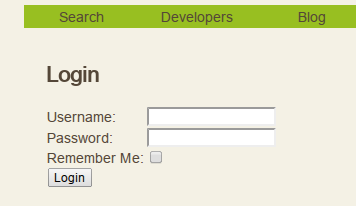
\includegraphics[width=0.5\textwidth]{../screenshots/login.png}
\end{center}

Hier ist der \emph{Loginbereich} der primär für \emph{Redakteure} interessant
ist die Beiträge auf der Blogseite veröffentlichen möchten. Auf der Loginseite
selbst ist kein weiterer zusätzlicher Content vorhanden.
\\
\\
Jeglicher Content in allen Kategorien wird ,,per Hand'' verfasst. Kopieren von
Texten ist verboten. Dadurch wollen wir die Orginalität unseres Contents
gewährleisten.

\section{Footer-Bereich}
In grafischer Hinsicht findet sich eine ,,Waldszene''. Diese haben wir vom 
,,Gnome Reference Manual'' \footnote{\url{http://developer.gnome.org/glib/}} übernommen.
Der Footer Bereich ist oben in der Übersicht abgebildet (Siehe
\ref{moosrdata_ref}).
Im \emph{Footer} befinden sich Links zu folgenden Seiten:

\paragraph{Social}
Im \emph{Social} Bereich befinden sich Links auf die folgenden sozialen Netze in
welche unsere Dienstleistung Vorganden ist:
\begin{itemize}
\item Flickr (Bildergallerien von Festivals und Community-Treffs, Bilder für den
    Blog)
\item Google+ (Unser Auftritt bei Google+)
\item Facebook (Unser Auftritt bei Facebook)
\item Twitter (Unser Microblogging Seite um kurz über Änderungen auf unserer
Seite zu informieren)
\item E-Mail Kontakt
\item RSS Feed zum Blog
\end{itemize}

Siehe auf der linken Seite in der Übersicht.
\\
\\
Wir haben uns bewusst für die Auslagerung von großen Bildergallerien auf Flickr
entschieden weil wir so Bilderreihen von Festivals oder Community-Treffs online
stellen können ohne dass hierbei Datenvolumen-Kosten auf unserer Seite
entstehen. Gleichzeitg sparen wir Speicherplatz auf unserem Server.
\\
\\
Die Einbindung von Flickr und den weiteren sozialen Netzen hat neben dem
,,Mundpropaganda Werbeeffekt'' den Vorteil, dass hier gleichzeitig ein
,,Hotspot'' auf unsere Seite generiert wird was unser Google Ranking verbessert.

\paragraph{Sitemap}
Die Sitemap bietet nochmal für den Google-Crawler die Möglichkeit in
alle wichtigen Bereiche unserer Seite zu kommen.
\paragraph{Featured Posts}
Unter ,,Featured Posts'' befinden sich einige von Hand ausgewählte Blogposts,
die hier verlinkt werden.

\paragraph{External Links}
Hier sind Links zu den von uns verwendeten Libraries wie z.B. libglyr. Dadurch
informieren wir nicht nur über die Technologien die wir verwenden sondern
ermöglichen es der Community auch indirekt an moosr über die Entwicklung an
Thirdparty-Libraries mitzuarbeiten.
\\
\\
Zudem finden sich hier externe Anbieter die unser Angebot ergänzen.
